% Chapter Template
% \doublespacing

\chapter{Introduction} % Main chapter title

\label{ChapterX} % Change X to a consecutive number; for referencing this chapter elsewhere, use \ref{ChapterX}

\lhead{Chapter I. \emph{Introduction}} % Change X to a consecutive number; this is for the header on each page - perhaps a shortened title

%----------------------------------------------------------------------------------------
%	SECTION 1
%----------------------------------------------------------------------------------------

\section{Rise of Unmanned Aerial Vehicles}
Unmanned aerial vehicles or UAVs have become ubiquitous in the past decade, both in research and industry. A myriad of applications involving UAVs in diverse fields has made them quite popular. Potential domestic  applications include Environmental monitoring and surveillance \cite{envmon}, traffic management \cite{trasur}, remote sensing \cite{remsen}, precision agriculture and farming \cite{preagr}, disaster management \cite{disman}, to name a few. The use of UAVs for defence purposes is only poised to grow in the next decade. It is not hard to see the appeal of UAVs in the defence sector with applications ranging from simple surveillance and reconnaissance missions to offensives like \textit{search and destroy} missions and targeted hits.

Much of the rise of this interest in UAVs can be attributed to associated advances in robotics, largely driven by the progress in robust and cheap sensors and communication technology. The emergence of scalable and extensible software architectures like the Robot Operating System(ROS), which enables easy integration of various subsystems further pushed the progress in these domains.

While early applications of UAVs were single UAV based, the focus is now shifting towards applications involving multiple UAVs, cooperatively completing tasks. There are several advantages of multi-UAV systems over single UAV systems. In certain applications like search and rescue missions, for instance, the use of multiple UAVs for surveying an area can significantly reduce the time taken to complete the task \cite{coosea}. As given by \cite{fanets}, other advantages of multi-UAV systems over single UAV systems include cost, scalability, survivability and speed.

Though UAV swarms have promising capabilities, they have quite a few challenges to overcome. Communication is one of the main hindrances to realize robust swarms of UAVs.

\section{The Challenge of Communications in UAV swarms}
While there is much literature regarding communication in UAV systems, \cite{fanets} and \cite{lavgupta} are two good survey articles regarding the current trends and issues in communication in UAV swarms. Besides pointing out the shifting interest towards multi UAV systems, due to their advantages over single UAV systems, they also identify the challenges in these systems, communication among the UAVs being the most notable one. 

Since the first applications were single UAV based, communication architecture in these systems was simple and straightforward. Often, there only needed to be a communication link between the UAV and the ground station. In some cases where the UAV has to cover a larger area, there could be multiple ground stations, and the UAV would have to communicate with the ground station near it. Even then, the overall architecture was pretty basic. As we noted earlier, there is a rapidly growing interest in realizing swarms of cooperative and collaborative UAVs, accomplishing complex tasks. Robust and reliable communication among the UAVs is an essential and critical component in enabling cooperative and collaborative behaviour in these UAV swarms.

While there is some interest in infrastructure based communication in UAVs, like using cellular infrastructure for UAVs \cite{celsur}, much of the research community considers enabling UAV communications in infrastructure less environments, more significant. These so called adhoc networks are important, for instance in disaster management scenarios where the existing infrastructure is damaged, or in military applications where there is no pre-existing infrastructure. The authors in \cite{lavgupta} try to identify several possible communication architectures for multi UAV networks.

\begin{figure}
	\centering
	\begin{subfigure}[b]{0.3\textwidth}
		\centering
		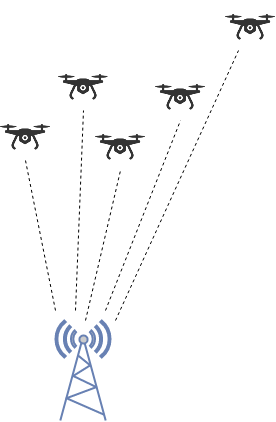
\includegraphics[scale=0.45]{Pictures/star.png}
		\caption{Star Configuration}
		\label{fig: starconf}
	\end{subfigure}
	\begin{subfigure}[b]{0.3\textwidth}
		\centering
		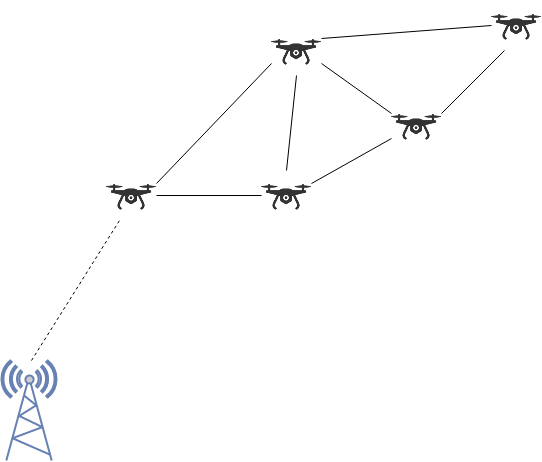
\includegraphics[scale=0.45]{Pictures/mesh.png}
		\caption{Mesh Configuration}
		\label{fig: meshconf}
	\end{subfigure}
	\caption{Possible network configurations for communications in UAVs}
	\label{fig: netconf}
\end{figure}

Figure \ref{fig: starconf} shows the star topology, where all the UAVs are connected to the ground station. In this configuration, the necessary communication among UAVs also needs to be routed through the ground station. Figure \ref{fig: meshconf} shows the mesh topology, where the UAVs communicate among themselves using an adhoc network, they themselves form. Typically, the ground station is also a part of the adhoc network.
